\documentclass{article}
% \documentclass[11pt]{amsart}
\usepackage[utf8]{inputenc}
\usepackage{amsmath,amsthm,amssymb,amsfonts,epic,epsfig,latexsym,enumerate}
% \usepackage{enumitem}
\usepackage[titlenotnumbered,linesnumbered,noend,plain]{algorithm2e} 
\usepackage{listings}
\usepackage{fullpage}
\usepackage{array}
\usepackage{mathtools}
\usepackage{xcolor}
\newtheorem{lemma}{Lemma}
\usepackage{url}
% \usepackage[dvipsnames]{xcolor}
\usepackage{tikz}
\usetikzlibrary{shapes,backgrounds}
\usepackage{epsfig} 		%Standard Macros
\usepackage{amssymb} 
\usepackage{amsmath}
\usepackage{tikz-cd}
% \usepackage[shortlabels]{enumitem}
\usepackage{pdfpages}
\usepackage{listings}
% \usepackage{multicol}

% \let\sitem\subitem
\def\sitem{\subitem $\Diamond$ }
\let\ssitem\subsubitem


\title{COM S 366: Ray Tracer Final Report}
\author{Ryan Leska}
\date{\today}

\begin{document}

\maketitle

\tableofcontents
\twocolumn





\section{General Information}

    This section is very wordy, I understand if you would like to skip it. \par
    generally its a desription of my usage of CUDA, parallelization, Importance Sampling, and Adaptive Sampling. As well as Information about my acceleration datastructure, and camera configuration. \par

    \subsection{CUDA}
    For my Ray Tracer (Path Tracer) Implementation, I decided to use CUDA c++ to parallelize the rendering process. This lead to a lot of headaches, dealing with memory issues and host-device scope issues, but in the end it seems to have sped up the rendering process significantly. \par

    The majority of my code runs on the device (gpu), but the host (cpu) is used to read in files like  textures and polygon meshes. The host is also used to write the final image to a file. \par  

    During testing I was able to run my program on a Nvidia 4070 ti and a Nvidia 3070 mobile. From this testing I determined that the best configuration for both of the gpus was to have 128 threads allocated per block (block count is calculated based on the number of pixels in the image). I generally chose to have my threads in a 16x8 because I believe that this increases the likelihood of cache hits. \par

        \subsubsection{CUDA Call Structure}
        First the main function allocates random number generators on the gpu (one for each thread). Then it reads in textures and polygon meshes on the host (cpu), then the data is allocated and copied to the gpu memory. The main function then allocates memory for the world and camera on the gpu. The world is then populated with hittables and materials. Then the render is ran on the gpu. After the render is complete the image data is copied from the gpu to the host and written to a file. \par



    \subsection{Sampling}



        \subsubsection{Implementation}
        The sampling method I settled on for my final implementation was a weight cosine hemisphere sample along side a weighted direct light sample. This method was chosen because it seemed to produce the best results in terms of noise and speed. \par
        When a scattering material is hit the ray has an equal (or configurable) chance to either scatter in a cosine weighted direction or towards a light. The light is chosen randomly from the list of lights in the world. Both of these samples are then weighted by their respective pdfs are applied to the final color. \par
        Due to my usage of CUDA my path tracing function getColor() is not recursive. Instead I used an iterative approach where the ray is scattered until it hits a light or the maximum depth is reached. \par 



        \subsubsection{Testing}
        During my testing I tried a bunch of different sampling methods. I tried a square random sample, a uniform sample, a cosine weighted sample, a power-weighted cosine sample, a Beckmann distribution sample, and a Blinn-Phong sample. I found that the a cosine weighted sample produced the best results in terms of lighting. Below is a test image I produced using each of these sampling methods. \par

        \begin{figure}[h]
            \centering
            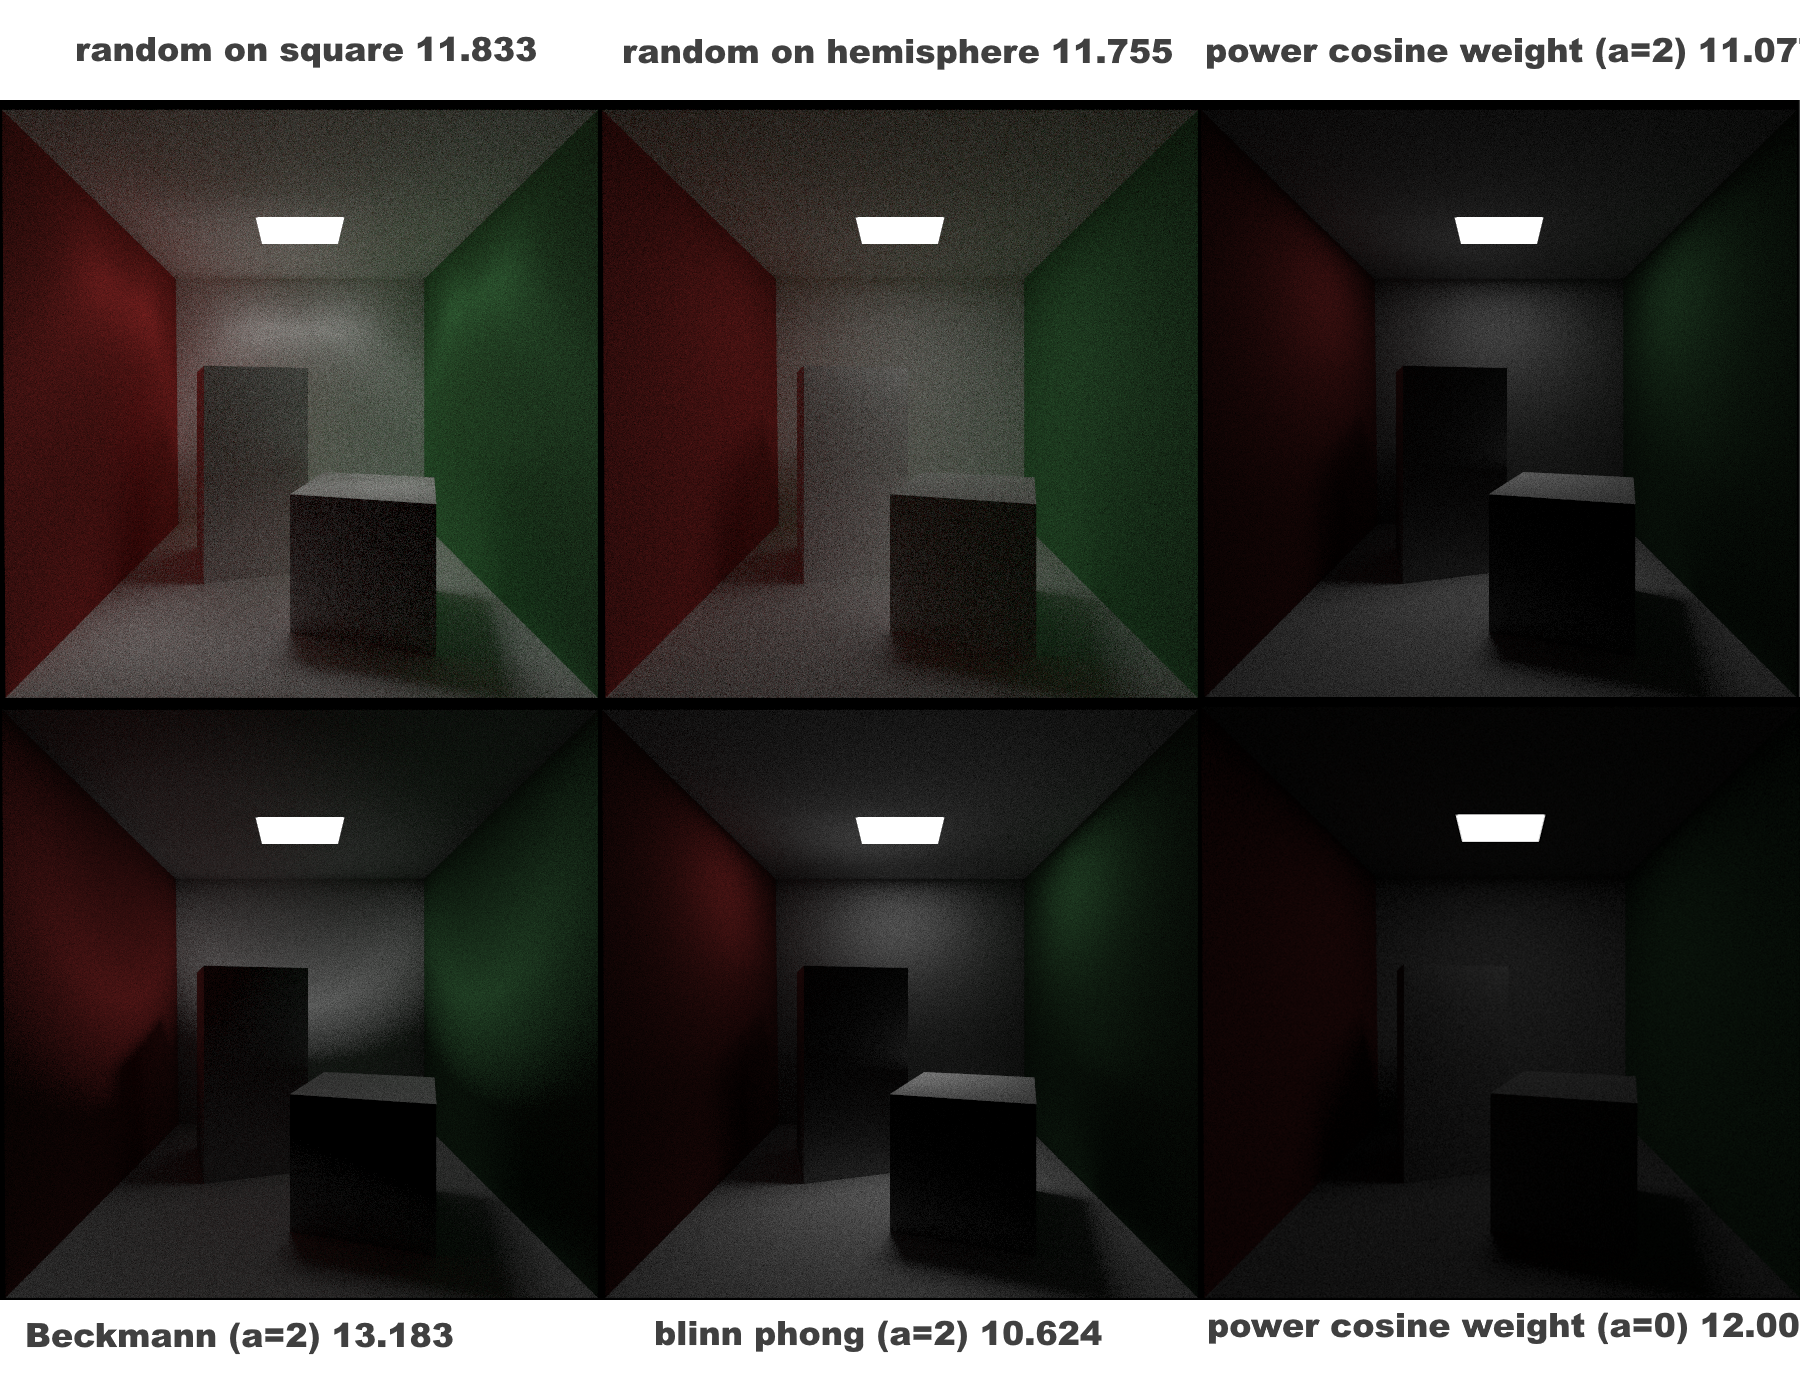
\includegraphics[width=0.5\textwidth]{samples/Lighting_Comparison.png}
            \caption{Sampling Test}
        \end{figure}


    \subsection{Octree - Acceleration Datastructure} 
    To help with the speed of my ray tracer I implemented an octree to store the hittables in the world. This octree is built when the world is created. Since I am using CUDA C++ I made the Octree a child of the scene (world) class. The octree is built by recursively splitting the world into 8 octants until the number of hittables in the octant is less than a threshold or a configurable depth is reached. \par 
    While working on the octree I though about how a voxel based render might be implemented to be really fast, so I might try that in the future. \par   




    \subsection{Camera Configuration}
    The camera is configured by setting a number of parameters during the world/camera creation. The camera is configured by setting the following parameters: \par
    \begin{enumerate}
        % \item resolution - the resolution of the image (width, height)
        \item fov - the field of view of the camera
        \item lookfrom - the position of the camera
        \item lookat - the position the camera is looking at
        \item vup - the up vector of the camera (used to determine the orientation of the camera)
        \item aspect ratio - the aspect ratio of the image (This can override the resolution)
        \item apature - the size of the apature (used to determine the depth of field)
        \item focus distance - the distance the camera is focused at (used to determine the depth of field)
        \item \quad
        \item MSAA - The scalar of samples per pixel when the camera detects an edge or aliased section 
        \item samples - The number of samples per pixel (pre-msaa)
        \item bounces - the number of bounces the ray will take before it is terminated
        \item Ambient Light - the percent brightness of the ambient light in the scene 
    \end{enumerate}



    \subsection{Anti-Aliasing - Adaptive Sampling}
    For Adaptive Sampling I implemented a method similar to MSAA that detects edge and aliased sections (like textures) and increases the number of samples taken in that area. This method is implemented by a simple edge detection algorithm in the hit function. If the hit function detects an edge or aliased section it will increase the number of samples taken in that area. \par


\section{Materials}



    \subsection{Lambertian}
    A lambertian material is a material that scatters light in all directions. This material is used to simulate a matte surface. \par


    \subsection{Metal}
    A metal material is a material that reflects light in a specular direction. This material is used to simulate a shiny surface (fuzzy or clear). \par



    \subsection{Dielectric}
    A dielectric material is a material that refracts light when it hits the surface. This material is used to simulate glass or water. \par



    \subsection{Textured}
    A textured material is a material that has a texture applied to it. This material is used to simulate surfaces with patterns or images. This material uses u,v mapping to determine the texture location. PPM textures are supported and must be read in by the cpu. \par



    \subsection{Light}
    A light material is a material that emits light. This material is used to simulate light sources in the scene. \par



    \subsection{Isotropic}
    An isotropic material is a material that scatters light in all directions. This material is used to simulate a matte surface. The way this differs from lambertian is that Isotropic sattering is in a sphere while lambertian is on the hemisphere \par



    \subsection{Other}



        \subsubsection{Phong}
        This material was lightly discussed in the class. I implemented it as a test, but it is not used in the final render. The material is a shaded material following the Phong Lighting model. \par



        \subsubsection{Phong-Lambertian}
        This material is a combination of a Phong and Lambertian material. The material is passed a parameter that determines a number of bounces before the material switches to a Phong material. This allows for the nice uniform phong lighting along with color bleeding and light reflections from nearby objects. This results in a similar result to Importance sampling with light sampling.\par

        
        \subsubsection{LambertianBordered}
        A lambertian material that returns a different color when an edge is hit. I created this during my testing of MSAA. I found the effect cool, its very similar to the cell shading seen in the video-game series Borderlands.\par



\section{Hittables}
    Hittable is misspelled in the code, I apologize for that. \par


    \subsection{Sphere}
    A sphere is a hittable object that is defined by a center and a radius.  \par


    \subsection{Polygons}
    A polygon is a hittable object that is defined by a list of vertices in a plane. I implemented this such that the polygons can be any number of vertices and these vertices can be texture mapped using u,v coordinates. \par


        \subsubsection{Triangle}
        To ease my scene creation I implemented a method Triangle that is passed 3 vertices and a material. This method creates a triangle from the vertices and material. \par


        \subsubsection{Rectangle}
        To ease my scene creation I implemented a method Rectangle that is passed 2 vertices and a material. This method creates a rectangle from the vertices and material. \par



    \subsection{Boxes}
    A box is a hittable object that is defined by a minimum and maximum point. \par



    \subsection{Continuous Medium}
    A continuous medium is a hittable object that is defined by a boundary and a density. This object can be used to simulate fog or smoke (using the isotropic material). \par



    \subsection{Object Instancing}
    Object Instancing are classes that are hittable in themsleves but contain other hittables. This allows for the creation of more complex objects from simpler objects. \par
    For each of the following classes I used ray inverse transformations to determine if a ray hit the object. \par


        \subsubsection{Translation}
        Translation is a class that is a hittable object that contains another hittable object. \par



        \subsubsection{Rotation}
        Rotation is a class that is a hittable object that contains another hittable object. \par



        \subsubsection{Motion Blur}
        Motion Blur is a class that is a hittable object that contains another hittable object. It is passed a Velocity vector, an Acceleration vector, and a time interval. The time interval determines both how far the object moves as well as the number of overall hit attempts per ray hit check. A long time leads to more sample and therefore a clearer movement (with respect to a lower time higher velocity).\par 



\section{Other Features}



    \subsection{Round Pixels}
    To make the image look better I implemented round pixels. When compiling the user can set a flag to either use a circular montecarlo sample (round pixel) or a square montecarlo sample (square pixel). \par


    \subsection{HDR}

\pagebreak
\section{Feature List Summary - For Easier Grading}

\begin{enumerate}[\quad]
    \item Required 
        \sitem Camera Configuration
            \ssitem Position, Orientation, Field of View
        \sitem Anti-Aliasing
            \ssitem configurable sample count 
            \ssitem See also Adaptive Sampling
        \sitem Ray/Sphere Intersection
        \sitem Ray/Triangle Intersection (Polygon)
        \sitem Load texture (PPM format)
        \sitem Textured Spheres and Triangle (both have u,v mapping)
        \sitem Acceleration Datastructure (Octree)
        \sitem Specular (Metal), Diffuse (Lambertian), and Dielectric Materials 
        \sitem Emissive Material (Light)
    \item For Points
        \sitem HDR (High Dynamic Range) 
        \sitem Volume Rendering (smoke, clouds)
        \sitem Quads (Rectangle, Box)
        \sitem Motion Blur 
        \sitem Defocus/Depth of Field (see camera configuration)
        \sitem Object Instancing (Translation, Rotation)
        \sitem Importance Sampling (Cosine weighted and Light Sampling)
        \sitem Round Pixels 
        \sitem Parallelization (CUDA)
        \sitem GPU Acceleration (CUDA)
        \sitem Adaptive Sampling (MSAA)   
    \item For Fun
        \sitem Phong lighting model 
        \sitem Phong-Lambertian Material
        \sitem LambertianBordered Material
        \sitem Other Sampling Methods (Beckmann, Blinn-Phong, Square, Uniform)   

\end{enumerate}

\end{document}